% reqno is needed to make the subnumcases have the case numbers on the right
\documentclass[reqno]{amsart}
% \documentclass{article}
% \documentclass[runningheads]{llncs}
% \documentclass[preview]{standalone}

\usepackage{mathtools}
\usepackage[english]{babel}
\usepackage{tabularx}
\usepackage{tikz}
\usepackage{xcolor}
% TODO: maybe get nicer colors
\definecolor{p1col1}{rgb}{1.0, 0, 0}
% \definecolor{p1col1}{RGB}{80, 0, 130}
\definecolor{p1col2}{rgb}{0, 1.0, 0}
% \definecolor{p1col2}{RGB}{255, 190, 10}
\definecolor{p1col3}{rgb}{0, 0, 1.0}
% \definecolor{p1col3}{RGB}{255, 190, 10}
\definecolor{p1col4}{rgb}{0, 0, 0}
\definecolor{lightpurple}{RGB}{203, 195, 227}
% \definecolor{p1col4}{RGB}{40, 0, 80}

\usepackage{graphicx}

\usepackage{verbatim}
\usepackage{amsfonts}
\usepackage{amssymb}
\usepackage{amsmath}

\usepackage{xcolor}
\usepackage{colortbl}

\usepackage{algorithm}
\usepackage[noend]{algpseudocode}


\usepackage{twoopt}
\usepackage{tikz}
\usepackage{tikz-qtree}
\usetikzlibrary{math}

\usepackage{caption}
\usepackage{subcaption}

\usepackage[title]{appendix}

\usepackage{verbatim}

\newcommand{\emptystring}{\varepsilon}

\usepackage{cases}





%
% Algorithm environment commands
%
% https://tex.stackexchange.com/questions/74880/algorithmicx-package-comments-on-a-single-line
\algnewcommand{\LineComment}[1]{\State \(\triangleright\) #1}

% https://tex.stackexchange.com/questions/184154/algorithmic-put-if-and-endif-into-same-line
\algnewcommand{\OneLineIf}[2]{\State\algorithmicif\ #1\ \algorithmicthen\ #2}

% https://tex.stackexchange.com/questions/234690/and-in-algorithm
\algnewcommand{\algorithmicand}{\textbf{ and }}
\algnewcommand{\algorithmicor}{\textbf{ or }}
\algnewcommand{\algorithmicnot}{\textbf{ not }}
\algnewcommand{\OR}{\algorithmicor}
\algnewcommand{\AND}{\algorithmicand}
\algnewcommand{\NOT}{\algorithmicnot}

\newcommand{\visit}[1]{\texttt{visit}(#1)}

% \newcommand{\pshift}[2][]{$\mathsf{preshift}_{#1}(#2)$}
\newcommand{\transpose}[3]{\mathsf{transpose(} #1, #2, #3 \mathsf{)}}
\newcommand{\preshift}[2]{\mathsf{preshift(} #1, #2 \mathsf{)}}

% \newcommand{\leftshift}[2]{\mathsf{leftshift(} #1, #2 \mathsf{)}}
\newcommand{\treeshift}[3]{\mathsf{shiftree(} #1, #2, #3 \mathsf{)}}


% https://tex.stackexchange.com/questions/228474/bold-horizontally-and-vertically-aligned-multiline-table-headers
\newcommand*{\thead}[1]{%
\multicolumn{1}{c}{\bfseries\begin{tabular}{@{}c@{}}#1\end{tabular}}}


    % TODO: might not actually need these
\newcommand{\leftshift}[3][]{\mathsf{left}_{#1}(#2,#3)}

\newcommand{\nextPrefix}[1]{\mathsf{next}{(#1)}}
\newcommand{\nextTree}[1]{\mathsf{nextree}{(#1)}}
\newcommand{\coolCat}[1]{\overrightarrow{\mathsf{coolCat}}{(#1)}}
\newcommand{\otree}[1]{\mathsf{OTree}{(#1)}}
\newcommand{\dyck}[1]{\mathsf{Dyck}{(#1)}}
\newcommand{\dyckindex}[1]{\mathsf{DyckIndex}{(#1)}}

\newcommand{\otreenode}[1]{\mathsf{OTreeNode}{(#1)}}
\newcommand{\leftdown}[1]{\mathsf{LD}{(#1)}}
\newcommand{\depth}[1]{\mathsf{Depth}{(#1)}}
% \newcommand{\ithone}[2]{\mathsf{i^{\underline{th}}one}_{#1}{(#2)}}
\newcommand{\ithone}[2]{\mathsf{i^{\underline{th}}one}({#1}, #2)}
\newcommand{\zeroesbetween}[3]{\mathsf{zeroesbetween({#1}, #2, #3)}}
\newcommand{\thh}{^{\underline{th}}}
% \newcommand{\thh}{Arnold Schwarzenegger}



\usepackage{tabularx,booktabs}
\usepackage[letterpaper,top=2cm,bottom=2cm,left=3cm,right=3cm,marginparwidth=1.75cm]{geometry}

\usepackage{amsmath}
\usepackage{graphicx}
\usepackage[colorlinks=true, allcolors=blue]{hyperref}

\title{Cooler than Cool: \\ Cool-Lex Order for Generating New Combinatorial Objects}
\author{Paul Lapey}


\begin{document}
\maketitle
\tableofcontents
% Two primary contributions, each with subcontributions
% each new result: one section on gray code, one section on implementation
% TODO: next meeting: each chapter heading set, at least some text for each chapter


% figure balanced parentheses binary trees
% add figures/exhaustive lists
\section{Combinatorial Generation: Looking at All the Possibilities}

Combinatorial generation is defined as the exhaustive listing of combinatorial objects of various types.  Frank Ruskey duly notes in his book \emph{Combinatorial Generation} that the phrase ``Let's look at all the possibilities" sums up the outlook of his book and the field as a whole \cite{ruskey2003combinatorial}. Examining all possibilities fitting certain criteria is frequently necessary in fields ranging from mathematics to chemistry to operations research. Combinatorial generation as an area of study seeks to find an underlying combinatorial structure to these possibilities and utilize it to obtain an algorithm to efficiently enumerate an appropriate representation of them \cite{ruskey2003combinatorial}. 

A quintessential result of the combinatorial generation in practice is Frank Gray's reflected binary code, or Gray code. Gray codes give a ``reflected" ordering of binary strings such that each successive string in the ordering differs from the previous string by exactly one bit. This contrasts from a lexicographic ordering of binary strings, in which a n-digit binary string can differ by up to n digits from its predecessor and will differ by approximately two (more precisely $\sum_{i=0}^n2^i$, which is 1.9375 for 4 bit values and 1.996 for 8 bit values) bits on average\footnote{Consecutive pairs of binary digits in lexicographic order will differ in the bit at position i with probability $\frac{1}{2^i}$.  Therefore, the average number of differing bits between two binary strings of length n is $\sum_{i=0}^n2^i$, which converges to 2 as n grows large.}. The binary reflected Gray code, therefore, provides an ordering that requires half as many bit switches on average as the more intuitive lexicographic order. Binary reflected Gray codes are widely used in electromechanical switches to reduce error and prevent spurious output associated with asynchronous bit switches.   The technique of reflecting all or certain parts of a string to generate new strings has become one of the most widely used techniques in combinatorial generation.
Crucially, Frank Gray's reflected binary code achieved a tangible benefit in error reduction through the use of an alternative method of enumerating binary strings.


\begin{figure}
    \centering
\includegraphics[width=4in]{BLX6-cropped.pdf} 

\includegraphics[width=4in]{BRGC6-cropped.pdf} 

\includegraphics[width=4in]{BCLX6-cropped.pdf} 

    \caption{Lexicographic (top), binary reflected Gray code (middle), and cool-lex (bottom) enumerations of 6-bit binary strings. \\ 
    Individual strings are read vertically with the most significant bit at the top; white is 1.
    }
    \label{binary}
\end{figure}

\section{Gray Codes for Other Objects} \label{sec:intro_Graycodes}
In this thesis, we are not concerned with counting combinatorial objects, but rather with efficiently ordering them.  We aim to create a \emph{Gray code} or \emph{minimal change ordering} for these objects.  Frank Gray's reflected binary code used complementing a single bit as the minimal change between successive binary strings in its ordering.  Other notions of minimal changes in strings are \emph{adjacent-transpositions}, or \emph{swaps}, which interchange two adjacent symbols in a string, and \emph{shifts}, in which a single symbol in a string moved to another position. Our Gray codes for strings will use a slightly more restrictive type of shift: a \emph{left-shift}, which moves a single symbol somewhere to the left within a string. 
% This means sequencing the objects such that each one differs from the other in a specific small way. For example, two successive integer strings might differ by shifting one symbol into another position, or two trees might differ by changing one node to be a child of a different node.
More specifically, if $\alpha = a_1 a_2 \ldots a_n$ is a string and $i < j$, then we let
\begin{equation}
    \lshiftindex[\alpha]{j}{i} = a_1 a_2 \ldots a_{i-1} a_j a_{i} a_{i+1} \ldots a_{j-1} a_{j+1} a_{j+2} \ldots a_n. \label{eq:leftdef}
\end{equation}


WHAT DOES IT MEAN TO HAVE A MINIMAL CHANGE ORDERING IN A TREE?

PICTURE? ESA IMAGE? BUT WITHOUT STACK?

MOVE LSHIFT DEF TO SEC 3?
NOT JUST OF THEORETICAL INTEREsT, VERY EFFICIENT


Our Gray code for ordered trees will use ``pops", which remove a node's first child, and ``pushes,'' which push one node to be the first child of another.  More specifically, the algorithm will generate trees using a pop-push operation that pops one node's first child and pushes it to become the first child of another node.  We will refer to this pop-push operation as a ``pull.''

% Our enumeration algorithms uses \emph{left shifts} and \emph{parent shifts}. Left shifts shift a single symbol in a string somewhere left (earlier) in the string; parent shifts shift a single node in a tree to be the first child of another node.

\section{Cool-Lex Order}

HAS BENEFITS OF LEX AND GRAY CODE
% connect Gray code and cool-lex order
Cool-lex order has introduced the idea of rotating sublists to enumerate languages.  Different versions of cool-lex order have been shown to enumerate several sets of combinatorial objects, including binary strings, fixed weight binary strings, Dyck words, and multiset permutations \cite{williams2009shift}.  Cool-lex orders often lead to algorithms that are faster and simpler than standard lexicographic order.  For example, the ``multicool" package in R uses a loopless cool-lex algorithm to efficiently enumerate multiset permutations.   The package started using cool-lex order for multiset permutations in versoin 1.1 and as of version 1.12 has been downloaded nearly a million times \cite{multicool_2021}.  A common thread in the cool-lex algorithms for combinatorial generation is their focus on the \emph{non-increasing prefix} of string, or the longest prefix of a string such that each successive symbol in the prefix is less than or equal to the previous symbol in the string.

\section{Goals of this Thesis}

% Cool-lex order has been shown to provide a minimal change cyclic ordering for Dyck words and binary trees. This thesis provides a new algorithm fo


This thesis will examine the use of cool-lex orders to enumerate other languages. Among these are ordered trees, Lukasiewicz words, and Motzkin words. 

This thesis will provide two primary contributions, each with sub-contributions.  

The first contribution is a `pop-push' Gray code for enumerating ordered trees in $O(1)$ time. Chapter \ref{chap:otree-graycode} will give a two-case successor rule for generating all ordered trees with $n$ nodes using at most two ``pull'' operations. Chapter \ref{chap:otree-implementation} will provide a loopless algorithm for the successor rule in \ref{chap:otree-graycode} and an implementation of the algorithm in C.

The second contribution is a shift Gray code for Lukasiewicz words.  Chapter \ref{chap:luka-graycode} will give a shift Gray code for generating Lukasiewicz words with fixed content using one prefix shift per iteration.  Chapter \ref{chap:luka-implementation} will give a loopless implementation of the algorithm in \ref{chap:luka-graycode} using an array based implementation for the special case of Motzkin words and a linked list implementation for the general case of unrestricted Lukasiewicz words.

Introduce all these things plus concepts/features that will be useful later.
The Catalan numbers are one of the most ubiquitous sequences of numbers in mathematics.  
Named for mathematician Eugene Charles Catalan, the $n\thh$ Catalan number can be succinctly defined as the number of ways of triangulating a convex polygon with $n+2$ sides.  Figure \ref{fig:pentagontriangulations} demonstrates this for the case of $n=3$ The sequence of Catalan numbers for $n \ge 0$ can be defined mathematically as follows:

\begin{align}
    \C_n &= \frac{(2n)!}{n!(n+1)!} =1, 1, 2, 5, 14, 42, 132, \ldots & \text{OEIS} A000108
\end{align}

\begin{figure}
\begin{center}
\begin{tikzpicture}
    \coordinate (a) at (-0,1);
    \coordinate (b) at (0.951,0.309);
    \coordinate (c) at (0.587,-0.809);
    \coordinate (d) at (-0.587,-0.809);
    \coordinate (e) at (-0.951,0.309);


\matrix[column sep=0.8cm,row sep=0.5cm]
{
    \pslice{a/d,a/c} &
    \pslice{b/e,b/d} &
    \pslice{c/a,c/e} &
    \pslice{d/b,d/a} &
    \pslice{e/c,e/b} \\
};
\end{tikzpicture}
\end{center}
    \caption{The $\C_3=5$ triangulations of a polygon with $3+2=5$ sides.}
\label{fig:pentagontriangulations}
\end{figure}
The Catalan numbers can also be expressed through a summation that hints at the recursive structure of many of the Catalan objects.  

\begin{align}
    \C_{n+1} &= \sum_{k=0}^{n}{\C_{k}\C_{n-k}} \textrm{,   }  \C_0=1
\end{align} 

In the case of triangulated polygons, this summation can be derived as follows:

$\C_{n+1}$ is the way of triangulating a convex polygon with $n+3$ sides.  Let $\mathcal{P}_{n+3}$ be a convex $(n+3)$-gon and let $\mathcal{T}$ be a triangulation of $\mathcal{P}_{n+3}$. Fix an edge $e$ in $\mathcal{P}_{n+3}$.  Note that $e$ lies between two vertices of $\mathcal{P}_{n+3}$. $e$ must be in exactly one triaingle in $\mathcal{T}$.  Let $T_{i}$ be the triangle in $\mathcal{T}$ that contains $e$.  $T_{i}$ must have two of its vertices on the two vertices of $e$ and one vertex that is another vertex in $\mathcal{P}_{n+3}$.  There are $n+1$ other vertices of $\mathcal{P}_{n+3}$.  Suppose the third vertex of $T_i$ is $k+1$ vertices clockwise of $e$, where $0\le k \le n$. Drawing $T_i$ divides $\mathcal{P}_{n+3}$ into 3 polygons: $T_i$, a $(k+2)$-gon clockwise of $T_i$, and a $(n-k+2)$-gon counterclockwise of $T_i$. This means that for each possible value of k, there is one way of triangulating $T_i$, $\C_k$ ways of triangulating the polygon clockwise of $T_i$, and $\C_{n-k}$ ways of triangulating the polygon counterclockwise of $T_i$.  Therefore, there are $C_k*C_{n-k}$ ways of triangulating $\mathcal{P}_{n+3}$ for each value of k.  Therefore, there are $\C_{n+1}=\sum_{k=0}^{n}{\C_{k}\C_{n-k}}$ total ways of triangulating $\mathcal{P}_{n+3}$. Figure \ref{fig:recursiveTriangulations} illustrates this process for the case of $n+1=6$.


The Catalan numbers count a remarkable number of interesting and useful combinatorial objects in bijective correspondence with triangulations of $n$-gons. Combinatorial objects counted by the Catalan numbers are referred to as \emph{Catalan objects}.   Richard Stanley's book \emph{Catalan Numbers} gives hundreds of examples of Catalan objects  as well as a thorough history on the numbers and their study \cite{stanley2015Catalan}. This thesis will focus primarily on three Catalan objects: Dyck words, binary trees, and ordered trees. 


\begin{figure}
    \centering
\begin{center}
\begin{tabular}{ c c c c c c c}
    \octoSliceTable{D} & \octoSliceTable{C}  & \octoSliceTable{B}  & \octoSliceTable{A}  & \octoSliceTable{H}  & \octoSliceTable{G}   \\
    $k=0$ & $k=1$ & $k=2$&$k=3$& $k=4$& $k=5$& \\
    2-gon; 7-gon & 3-gon; 6-gon& 4-gon; 5-gon&5-gon; 4-gon & 6-gon; 3-gon& 7-gon; 2-gon& \\
    $\C_0 *\C_5$ & $\C_1 *\C_4$&$\C_2 *\C_3$ & $\C_3 *\C_2$&$\C_4 *\C_1$ & $\C_5 *\C_0$ \\

    $1 *42$ & $1 * 14$&$2*5$ & $5*2$&$14*1$ & $42*1$ \\
    $42$ & $14$ & $10$ & $10$ & $14$ & $42$
\end{tabular}

\bigskip


$C_6=\sum_{k=0}^5\C_k\C_{n-k}=42 + 14 + 10 + 10 + 14 + 42 = 132$
\end{center}
    \caption{Constructing $\C_6$, the number of ways to triangulate an octagon, from triangulations of smaller sub-polygons.}
    \label{fig:recursiveTriangulations}
\end{figure}
\section{Dyck Words and Paths} \label{sec:Dycks}

The language of binary Dyck words is the set of binary strings that satisfy the following conditions: The string has an equal number of ones and zeroes and each prefix of the string has at least as many ones as zeroes.  The number of distinct Dyck words with $n$ ones and $n$ zeroes is equal to $\C_n$.  Dyck words with $n$ ones and $n$ zeroes are frequently referred to as Dyck words of \emph{order n}.
For example, the $\C_2=2$ Dyck words of order 2 are $1100$ and $1010$.

% TODO: don't love this phrasing
Two common interpretations of Dyck words are balanced parentheses and paths in the Cartesian plane. If each one in a Dyck word is taken to represent an open parenthesis and each zero a closing parenthesis, the Dyck language becomes the language of balanced parentheses.  Alternatively, the Dyck language can be interpreted as the set of paths in the Cartesian plane using $(1,1)$ (northeast) and $(1,-1)$ (southeast) steps that start at $(0,0)$, end at $(0,0)$ and never go below the x axis. In this case, each one in a Dyck word represents a $(1,1)$ step and each zero represents a $(1,-1)$ step.

Figure $\ref{fig:Dycks}$ gives an illustration of each of these interpretations of Dyck words for $n=4$.

\begin{figure}[H]
    \centering
    % This figure is temporarily omitted because it is slow
    \begin{tabularx}{0.55\textwidth}{>{\hsize=0.4\hsize}C >{\hsize=0.2\hsize}C >{\hsize=0.2\hsize}C   }
       \thead{Dyck Path} & \thead{Dyck Word} & \thead{Parentheses} \\ \hline 
\DyckTable[4]{2,2,2,2,0,0,0,0} & 11110000 & (((())))\\
\DyckTable[3]{2,0,2,2,2,0,0,0} & 10111000 & ()((()))\\
\DyckTable[3]{2,2,0,2,2,0,0,0} & 11011000 & (()(()))\\
\DyckTable[3]{2,2,2,0,2,0,0,0} & 11101000 & ((()()))\\
\DyckTable[2]{2,0,2,2,0,2,0,0} & 10110100 & ()(()())\\
\DyckTable[2]{2,2,0,2,0,2,0,0} & 11010100 & (()()())\\
\DyckTable[2]{2,0,2,0,2,2,0,0} & 10101100 & ()()(())\\
\DyckTable[2]{2,2,0,0,2,2,0,0} & 11001100 & (())(())\\
\DyckTable[3]{2,2,2,0,0,2,0,0} & 11100100 & ((())())\\
\DyckTable[2]{2,0,2,2,0,0,2,0} & 10110010 & ()(())()\\
\DyckTable[2]{2,2,0,2,0,0,2,0} & 11010010 & (()())()\\
\DyckTable[1]{2,0,2,0,2,0,2,0} & 10101010 & ()()()()\\
\DyckTable[2]{2,2,0,0,2,0,2,0} & 11001010 & (())()()\\
\DyckTable[3]{2,2,2,0,0,0,2,0} & 11100010 & ((()))()\\
    \end{tabularx}
    \caption{The $\C_4=14$ Dyck words of order 4}
    \label{fig:Dycks}
\end{figure}

\section{Binary Trees}

Binary trees are fundamental objects in computer science, and are commonly used for searching, sorting, and storing data hierarchically. A binary tree can be defined recursively as follows: The empty set $\phi$ is a binary tree. Otherwise a binary tree has a root vertex, a left subtree, and a right subtree, where each subtree is also a binary tree. A closely related object is an \emph{extended binary tree}, which is a binary tree for which every non-leaf node has exactly two children.  

Binary trees and extended binary trees are both counted by the Catalan numbers: $\C_n$ is the number of binary trees with $n$ nodes and the number of extneded binary trees with $n$ internal nodes.  
A binary tree $b$ with $n$ nodes can be constructed from an extended binary tree $e$ with n internal nodes by removing all leaves from the extended binary tree, leaving the $n$ internal nodes as the only remaining nodes.

This process can be reversed to construct an extended binary tree with $n$ internal nodes from a binary tree with $n$ nodes. Given a binary tree $b$ with $n$ nodes, add two leaf children to every leaf in $b$ and add one leaf child to every node in $b$ with one child. Following these steps, every node originally in $b$ is now an internal node, and therefore the constructed tree is an extended binary tree with n internal nodes.

\section{Ordered Trees}

An ordered tree is a tree for which each node can have an unrestricted number of children and the order of a node's children is significant.  An ordered tree can be defined recursively as follows:


An ordered tree is a tuple $(r,C)$ where $r$ is a root node and $C$ is either the empty set $\phi$ or an ordered sequence of children $(P_1\dots P_m)$ where each $P_i$ is an ordered tree.  Because of the designation of $r$ as a root vertex, an ordered tree cannot be empty, unlike a binary tree.

The number of ordered trees with $n+1$ nodes is equal to $\C_n$.

\begin{figure}
    \begin{subfigure}[]{\textwidth}
	\centering
\begin{tikzpicture}[every tree node/.style={draw,circle},sibling distance=6, level distance=20]
\tikzset{every tree node/.style={minimum width=1.4em,draw,circle},
         blank/.style={draw=none},
         edge from parent/.style=
         {draw,edge from parent path={(\tikzparentnode) -- (\tikzchildnode)}},
         level distance=1.5cm}
    \Tree [.{} [.{} [.{} \edge[draw=none]; \node[blank]{};\edge[draw=none]; \node[blank]{};] \edge[draw=none]; \node[blank]{};] \edge[draw=none]; \node[blank]{};] 
\end{tikzpicture}
\begin{tikzpicture}[every tree node/.style={draw,circle},sibling distance=6, level distance=20]
\tikzset{every tree node/.style={minimum width=1.4em,draw,circle},
         blank/.style={draw=none},
         edge from parent/.style=
         {draw,edge from parent path={(\tikzparentnode) -- (\tikzchildnode)}},
         level distance=1.5cm}
    \Tree [.{} \edge[draw=none]; \node[blank]{};[.{} [.{} \edge[draw=none]; \node[blank]{};\edge[draw=none]; \node[blank]{};] \edge[draw=none]; \node[blank]{};] ] 
\end{tikzpicture}
\begin{tikzpicture}[every tree node/.style={draw,circle},sibling distance=6, level distance=20]
\tikzset{every tree node/.style={minimum width=1.4em,draw,circle},
         blank/.style={draw=none},
         edge from parent/.style=
         {draw,edge from parent path={(\tikzparentnode) -- (\tikzchildnode)}},
         level distance=1.5cm}
    \Tree [.{} [.{} \edge[draw=none]; \node[blank]{};[.{} \edge[draw=none]; \node[blank]{};\edge[draw=none]; \node[blank]{};] ] \edge[draw=none]; \node[blank]{};] 
\end{tikzpicture}
\begin{tikzpicture}[every tree node/.style={draw,circle},sibling distance=6, level distance=20]
\tikzset{every tree node/.style={minimum width=1.4em,draw,circle},
         blank/.style={draw=none},
         edge from parent/.style=
         {draw,edge from parent path={(\tikzparentnode) -- (\tikzchildnode)}},
         level distance=1.5cm}
    \Tree [.{} \edge[draw=none]; \node[blank]{};[.{} \edge[draw=none]; \node[blank]{};[.{} \edge[draw=none]; \node[blank]{};\edge[draw=none]; \node[blank]{};] ] ] 
\end{tikzpicture}
\begin{tikzpicture}[every tree node/.style={draw,circle},sibling distance=6, level distance=20]
\tikzset{every tree node/.style={minimum width=1.4em,draw,circle},
         blank/.style={draw=none},
         edge from parent/.style=
         {draw,edge from parent path={(\tikzparentnode) -- (\tikzchildnode)}},
         level distance=1.5cm}
    \Tree [.{} [.{} \edge[draw=none]; \node[blank]{};\edge[draw=none]; \node[blank]{};] [.{} \edge[draw=none]; \node[blank]{};\edge[draw=none]; \node[blank]{};] ] 
\end{tikzpicture}

	\caption{The $\C_3=5$ binary trees with 3 nodes}
	\label{fig:binarytrees}
	\label{fig:}
    \end{subfigure}
    \begin{subfigure}[]{\textwidth}
	\centering
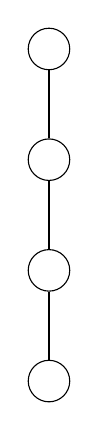
\begin{tikzpicture}[every tree node/.style={draw,circle},sibling distance=10pt, level distance=40pt]
\tikzset{minimum width=1.5em,edge from parent/.style={draw, edge from parent path=
    {(\tikzparentnode) -- (\tikzchildnode)}}}
    \Tree [.{} [.{} [.{} [.{} ] ] ] ] 
\end{tikzpicture} \hspace{2.9em}
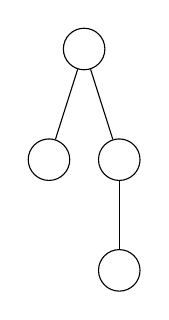
\begin{tikzpicture}[every tree node/.style={draw,circle},sibling distance=10pt, level distance=40pt]
\tikzset{minimum width=1.5em,edge from parent/.style={draw, edge from parent path=
    {(\tikzparentnode) -- (\tikzchildnode)}}}
    \Tree [.{} [.{} ] [.{} [.{} ] ] ] 
\end{tikzpicture} \hspace{2.9em}
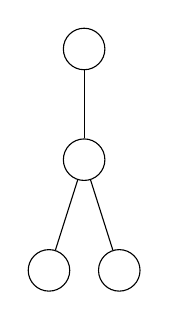
\begin{tikzpicture}[every tree node/.style={draw,circle},sibling distance=10pt, level distance=40pt]
\tikzset{minimum width=1.5em,edge from parent/.style={draw, edge from parent path=
    {(\tikzparentnode) -- (\tikzchildnode)}}}
    \Tree [.{} [.{} [.{} ] [.{} ] ] ] 
\end{tikzpicture} \hspace{2.9em}
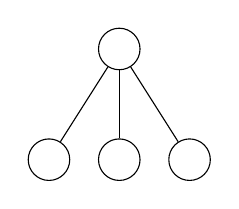
\begin{tikzpicture}[every tree node/.style={draw,circle},sibling distance=10pt, level distance=40pt]
\tikzset{minimum width=1.5em,edge from parent/.style={draw, edge from parent path=
    {(\tikzparentnode) -- (\tikzchildnode)}}}
    \Tree [.{} [.{} ] [.{} ] [.{} ] ] 
\end{tikzpicture} \hspace{2.9em}
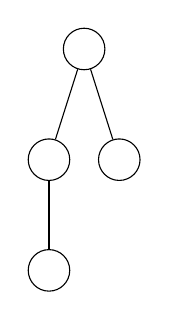
\begin{tikzpicture}[every tree node/.style={draw,circle},sibling distance=10pt, level distance=40pt]
\tikzset{minimum width=1.5em,edge from parent/.style={draw, edge from parent path=
    {(\tikzparentnode) -- (\tikzchildnode)}}}
    \Tree [.{} [.{} [.{} ] ] [.{} ] ] 
\end{tikzpicture}
	\caption{The $\C_3=5$ ordered trees with $3+1=4$ nodes}
	\label{fig:otrees}
    \end{subfigure}
\end{figure}



\section{Bijections}

Since Dyck Words, binary trees, and ordered trees are all Catalan objects, all three sets of objects are in bijective correspondence with each other.  For convenience, we will use the $\mathbf{D}_n$, $\mathbf{B}_n$, $\mathbf{E}_n$, and $\mathbf{T}_n$ to refer to the set of Dyck words of order $n$, the set of binary trees with $n$ nodes, the set of extended binary trees with $n$ internal nodes, and the set of ordered trees with $n+2$ nodes respectively.  

\subsection{Binary Trees and Dyck Words}

The bijection between extended binary trees and Dyck words is particularly elegant: 
For any $e \in \mathbf{E}_n$, traverse e in preorder.  Record a $1$ for each internal node; record a $0$ for each leaf ignoring the final leaf. The resulting binary sequence is a Dyck word  $D \in \mathbf{D}_n $ corresponding to the extended binary tree $e$.  This process can be reversed to go from $\mathbf{D}_n$ to $\mathbf{E}_n$.

\begin{figure}
    \centering
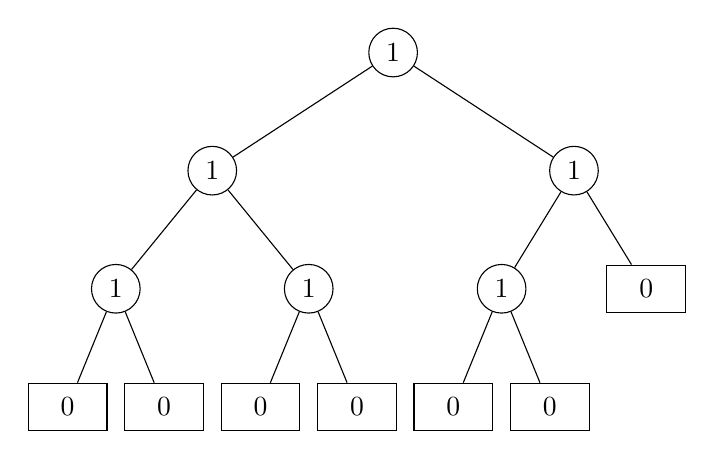
\begin{tikzpicture}[every tree node/.style={draw,circle},sibling distance=6, level distance=20]
\tikzset{every tree node/.style={minimum width=1.5em,draw,circle},
         blank/.style={draw=none},
         edge from parent/.style=
         {draw,edge from parent path={(\tikzparentnode) -- (\tikzchildnode)}},
         level distance=1.5cm}
    \Tree [.{1} [.{1} [.{1} [.\node[style={rectangle,minimum height=.6cm,minimum width=1cm}]{0}; ][.\node[style={rectangle,minimum height=.6cm,minimum width=1cm}]{0}; ]] [.{1} [.\node[style={rectangle,minimum height=.6cm,minimum width=1cm}]{0}; ][.\node[style={rectangle,minimum height=.6cm,minimum width=1cm}]{0}; ]] ] [.{1} [.{1} [.\node[style={rectangle,minimum height=.6cm,minimum width=1cm}]{0}; ][.\node[style={rectangle,minimum height=.6cm,minimum width=1cm}]{0}; ]] [.\node[style={rectangle,minimum height=.6cm,minimum width=1cm}]{0}; ]] ] 
\end{tikzpicture} \hspace{1em}
\begin{tikzpicture}[every tree node/.style={draw,circle},sibling distance=6, level distance=20]
\tikzset{every tree node/.style={minimum width=1.5em,draw,circle},
         blank/.style={draw=none},
         edge from parent/.style=
         {draw,edge from parent path={(\tikzparentnode) -- (\tikzchildnode)}},
         level distance=1.5cm}
    \Tree [.{} [.{} [.{} \edge[draw=none]; \node[blank]{};\edge[draw=none]; \node[blank]{};] [.{} \edge[draw=none]; \node[blank]{};\edge[draw=none]; \node[blank]{};] ] [.{} [.{} \edge[draw=none]; \node[blank]{};\edge[draw=none]; \node[blank]{};] \edge[draw=none]; \node[blank]{};] ] 
\end{tikzpicture}
    \caption{The extended binary tree (left) and binary tree (right) corresponding to the Dyck word 111001001100 \\
    Note that a preorder traversal of the extended binary tree excluding its final leaf yields 111001001100.
    }
\label{fig:binarytreesbijection}
\end{figure}


\subsection{Ordered Trees and Dyck Words} \label{subsec:otree-dyck-bij}
The bijection between ordered trees and Dyck words is particularly relevant to this paper's results, as it is central to the loopless ordered tree generation algorithm given in Chapter \ref{chap:otree-graycode}.
This algorithm will use the bijection between ordered trees and Dyck words specified in Richard Stanley's \emph{Catalan Objects} \cite{stanley2015Catalan}. Figure \ref{ordered_tree_bijection_illustration} illustrates both directions of the bijection.
The bijection can be formalized as follows:
\footnote{ Stanley's text refers to ordered trees as \emph{plane trees} and Dyck words as \emph{ballot sequences}} 


Given an ordered tree T with $n+1$ nodes: Traverse T in preorder.  Whenever going ``down" an edge, or away from the root, record a 1.  Whenever going ``up" an edge, or towards the root, record a 0.  The resulting binary sequence is a Dyck word D corresponding to the ordered tree T. 

This process can be inverted as follows: 

Let $D=d_1...d_{2n}$ be a Dyck word of order $n$ with $n > 0$. Construct an ordered tree T via the following steps. 

Let T be an ordered tree with root $r$.  Keep track of a current node $c$ and set $c$ equal to the root $r$.

\begin{itemize}
    \item For each $d_i$ such that $1 \le i \le 2n$ 
	\begin{itemize}
	    \item if $d_i=1$, then add a rightmost child $ch$ to $c$'s children; set $c=ch$
	    \item if $d_i=0$, then set $c$ equal to $c$'s parent.
	\end{itemize}
	%TODO: QUESTION: do I need to prove this? It seems like Stanely assumed this was basically obvious 

\end{itemize}

Following the execution of these steps, $r$ is the root of an ordered tree with $n$ nodes corresponding to the Dyck word $D$.

\begin{figure}
    \centering
    \includegraphics[width=0.5\textwidth]{otreebij.png}
    \caption{An ordered tree with $6+1=7$ nodes corresponding to the order 6 Dyck word $110101001100$.}
    \label{ordered_tree_bijection_illustration}
\end{figure}


\chapter{Loopless Ordered Tree Generation} \label{chap:otree}
This chapter presents the first loopless algorithm for generating all ordered trees with n nodes. 
% Cooldyck was first loopless for Dyck and Binary; we now show also ordered
% Give exampl  of bit change that messup tree (show for bin and o). 
% \chapter{Test}

Ruskey and Williams previously gave a cool-lex algorithm for looplessly generating all Dyck words  of a given length via prefix shifts \cite{ruskey2008generating}.  In the same paper, Ruskey and Williams also gave a loopless algorithm for generating all binary trees with a fixed number in the same order.

% TODO: rephrase 
% In this thesis, we consider ordered trees cool lex, it's minimal change and loopless. this is not nec true for any dyck word minimal change order. One order, 3 loopless algorithms for 3 coolest catalan structures. 
% This thesis provides an additional adaptation of the successor rule to looplessly generating ordered trees with a fixed number of nodes via node shifts. % reasonable term?
% TODO: adaptation of order, new successor rule
This thesis provides a new algorithm that generates ordered trees with a fixed number of nodes in a cool-lex order. The algorithm generates a minimal change ordering of ordered trees in the same order as their corresponding Dyck words in Ruskey and Williams's paper. Like the cool-lex algorithms for Dyck words and binary trees, this algorithm can be implemented looplessly: each ordered tree takes worst-case constant time to generate. This is faster than other algorithms for generating ordered trees which take constant amortized time \cite{parque2021efficient} \cite{er1985lexotrees} \cite{zaks1980lexotrees} \cite{skarbek1988pointerotrees}. Moreover, taken in conjunction with Ruskey and Williams's algorithms for Dyck words and binary trees, this algorithm completes a trio of loopless cool-lex algorithms for enumerating the three foremost Catalan structures.


% can't actually say this, unfortunately
Parque and Miyashita present a constant amortized time algorithm for generating ordererd trees, claiming that it operates ``with utmost efficiency'' \cite{parque2021efficient}.  Our algorithm operates in worst-case constant time per tree, which is faster. To borrow Parque and Miyashita's terminology, perhaps we should say that our algorithm operates with \emph{utmoster} efficiency

Like the cool-lex algorithm for binary trees, this algorithm generates ordered trees stored as pointer structures.  This contrasts from other efficient gray codes for enumerating ordered trees, which use either bit-strings or integer sequences to represent ordered trees \cite{parque2021efficient} \cite{zaks1980lexotrees} \cite{er1985lexotrees} as representations of ordered trees.  Skarbek's 1988 paper \emph{Generating Ordered Trees} gives a constant amortized time algorithm for generating ordered trees stored as pointer structures and is therefore a a noable exception to this \cite{skarbek1988pointerotrees}.
Generating ordered trees via a pointer structure facilitates the practical %TODO: word?
use of the trees generated by this algorithm, as a translation step between an alternative representation and a tree structure to traverse the tree is not necessary.


\section{Successor Rule}

Let $F$ be the leftmost leaf of T, or equivalently the leftmost descendant of the root. Consider the unique path between the root of T and $F$, denoted $\path{T}{root}{F}$. We will refer to this path as the left-down path of T, or $\leftdown{T}$

% path to leftmost descendent
% Define the left-down path of an ordered tree T, denoted $\leftdown{T}$ to be the first $s+1$ nodes in a preorder traversal of T such that, for each $t_i$ with $0 \le i \le s$, $i=0$ or $t_i$ is the leftmost child of $t_{i-1}$.

Given an ordered tree T, let O be the first node in a preorder traversal of T that is not in the $\path{T}{root}{F}$. If $\path{T}{root}{F}=T$, i.e. the entire tree is a single path, let O be the leaf of the tree. Let P be O's parent.  Let G be P's parent, and let L be P's leftmost child (or, equivalently, O's left sibling).  The labels P, G, and L are mnemonics for O's (p)arent, (g)randparent, and (l)eft sibling. 
Fig. \ref{exampleotree} gives an example illustrating O,P,G,L,F, and the left-down path in an tree.
\begin{figure}
    \centering
    $T=$

    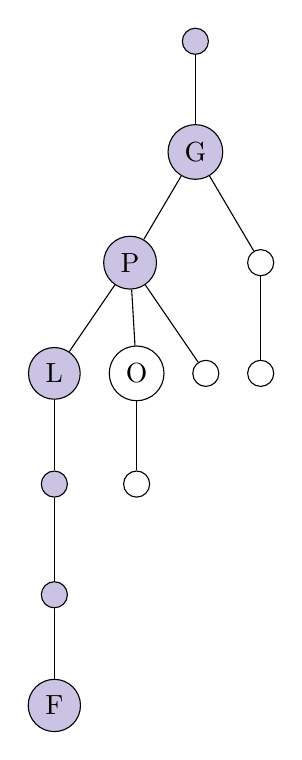
\begin{tikzpicture}[every tree node/.style={draw,circle},sibling distance=10pt, level distance=40pt]
	\tikzset{edge from parent/.style={draw, edge from parent path=
	{(\tikzparentnode) -- (\tikzchildnode)}}}
	\Tree [.\node[style={fill=lightpurple}]{}; [.\node[style={fill=lightpurple}]{G}; [.\node[style={fill=lightpurple}]{P};[.\node[style={fill=lightpurple}]{L}; [.\node[style={fill=lightpurple}]{}; [.\node[style={fill=lightpurple}]{}; [.\node[style={fill=lightpurple}]{F}; ] ] ] ] [.\node{O}; [.\node{}; ] ] [.\node{}; ] ] [.\node{}; [.\node{}; ] ] ] ]
    \end{tikzpicture}

    $D=[1, 1, 1, 1, 1, 1, 0, 0, 0, 0, 1, 1, 0, 0, 1, 0, 0, 1, 1, 0, 0, 0]$
    \caption{An ordered tree with 12 nodes corresponding to the Dyck word 1111110000110010011000.  The left down path of T is highlighted in purple. }
    \label{exampleotree}
\end{figure}

% Given an ordered tree T, let $\treeshift{T}{A}{B}$ be a function that shifts A to be the first child of B, with the restriction that A is a \emph{first-born}s, or the first child of its parents.
Given an ordered tree T and an ordered tree node A in T, let $\popchild{A}$ be a function that removes and returns A's first child.  In other words, it pops A's first child.  

Additionally, let $\pushchild{A}{B}$ be a function that makes B A's first child.  In other words, it pushes B onto A's list of children. 

For convenience, we will also define $\poppush{A}{B}=\pushchild{B}{\popchild{A}}$, which removes the first child of A and makes it the new first child of B.

The successor rule for enumerating ordered trees with n nodes can be stated as folows:

% $$
\bigskip


% $\popchild{O}$

% \begin{subnumcases}{\nextTree{T} = \label{eq:otreeRule}}
%     % \treeshift{\treeshift{T}{L}{G}}{O}{root}& if $P \ne root $ and O has no children \label{eq:otree_zeroshift}\\
%     \pushchild{O}{\popchild{P}} &  $P \ne root $ and O has no children \label{eq:otree_zeroshift}\\
%     \pushchild{G}{\popchild{P}};\pushchild{root}{\popchild{P}}  &  otherwise\label{eq:otree_oneshift} \\
%     % & otherwise \nonumber
%     % a &  
%     % \treeshift{T}{L}{O} & otherwise \label{eq:otree_oneshift}
% \end{subnumcases}

\begin{subnumcases}{\nextTree{T} = \label{eq:otreeRule}}
    \poppush{P}{G};\poppush{P}{root}  &  $P \ne root $ and O has no children \label{eq:otree_zeroshift}\\
    \poppush{P}{O} &  otherwise\label{eq:otree_oneshift}
\end{subnumcases}



Figure \ref{fig:otreeruledemo} gives a demonstration of the shifts in cases \ref{eq:otree_zeroshift} and \ref{eq:otree_oneshift}


To make the order cyclic, an additional rule can be added, modifying the successor rule to be:

\begin{subnumcases}{\nextTree{T} = \label{eq:otreeRule_cyclic}}
    \poppush{P}{root} &  $\leftdown{T}=T$ \label{eq:otree_noo_cyclic}\\
    \poppush{P}{G};\poppush{P}{root}  &  $P \ne root $ and O has no children \label{eq:otree_zeroshift_cyclic}\\
    \poppush{P}{O} &  otherwise\label{eq:otree_oneshift_cyclic}
\end{subnumcases}

% \begin{subnumcases}{\nextTree{T} = \label{eq:otreeRule_cyclic}}
%     \treeshift{T}{F}{root} & $\leftdown{T}=T$ \label{eq:otree_noo_cyclic}\\
%     \treeshift{\treeshift{T}{L}{G}}{O}{root}& if $P \ne root $ and O has no children \label{eq:otree_zeroshift_cyclic}\\
%     \treeshift{T}{L}{O} & otherwise \label{eq:otree_oneshift_cyclic}
% \end{subnumcases}

\begin{figure}
    \begin{subfigure}[]{.5 \textwidth}
	\begin{center}
	    11111000100100 $\implies$ 10111100010100

	    \begin{tikzpicture}[every tree node/.style={draw,circle},sibling distance=10pt, level distance=40pt]
		\tikzset{edge from parent/.style={draw, edge from parent path=
		{(\tikzparentnode) -- (\tikzchildnode)}}}
		\Tree [.{} [.\node[style={fill=lightyellow}]{G}; [.\node[style={fill=lightpurple}]{P}; [.\node[style={fill=pink}]{L}; [.{} [.{} ] ] ] [.\node[style={fill=lightblue}]{O}; ] ] [.{} ] ] ]
	    \end{tikzpicture}
	    $\implies$
	    \begin{tikzpicture}[every tree node/.style={draw,circle},sibling distance=10pt, level distance=40pt]
		\tikzset{edge from parent/.style={draw, edge from parent path=
		{(\tikzparentnode) -- (\tikzchildnode)}}}
		\Tree [.{} [.\node[style={fill=lightblue}]{O}; ] [.\node[style={fill=lightyellow}]{G}; [.\node[style={fill=pink}]{L}; [.{} [.{} ] ] ] [.\node[style={fill=lightpurple}]{P}; ] [.{} ] ] ]
	    \end{tikzpicture}
	\end{center}
	\caption{$O$ has no children, $P \ne root$: \\
	$\poppush{P}{G};\poppush{P}{root}$ \\
	$L$ becomes $G$'s first child; \\
	$O$ becomes the first child of $root$\\
	% test
	}
	\label{fig:}
    \end{subfigure}
    \begin{subfigure}[]{.5 \textwidth}
	\begin{center}
	    11110001100100 $\implies$ 11111000100100

	    \begin{tikzpicture}[every tree node/.style={draw,circle},sibling distance=10pt, level distance=40pt]
		\tikzset{edge from parent/.style={draw, edge from parent path=
		{(\tikzparentnode) -- (\tikzchildnode)}}}
		\Tree [.{} [.\node[style={fill=lightpurple}]{P}; [.\node[style={fill=pink}]{L}; [.{} [.{} ] ] ] [.\node[style={fill=lightblue}]{O}; [.{} ] ] [.{} ] ] ]
	    \end{tikzpicture} $\implies$
	    \begin{tikzpicture}[every tree node/.style={draw,circle},sibling distance=10pt, level distance=40pt]
		\tikzset{edge from parent/.style={draw, edge from parent path=
		{(\tikzparentnode) -- (\tikzchildnode)}}}
		\Tree [.{} [.\node[style={fill=lightpurple}]{P}; [.\node[style={fill=lightblue}]{O}; [.\node[style={fill=pink}]{L}; [.{} [.{} ] ] ] [.{} ] ] [.{} ] ] ]
	    \end{tikzpicture}
	\end{center}
	\caption{$O$ has at least 1 child \\
	$\poppush{P}{root}$ \\
	$L$ becomes $O$'s first child
	}
	\label{fig:}
    \end{subfigure}

    % TODO: change bit colors
    \caption{Illustrations of cases \ref{eq:otree_zeroshift} and \ref{eq:otree_oneshift} }
    \label{fig:otreeruledemo}
\end{figure}

% \begin{figure}[]
% 	\centering

% 	\caption{}
% 	\label{}
% \end{figure}

The following remarks can be derived from from the definition of the successor role and the nodes O,G,L, and T.


Let $D=\dyck{T}$; $s$ be the number of consecutive ones to start D, and $z$ be the number of consecutive zeroes starting at $d_{s+1}$.  Note that $z=(k-s-1)$; $d_{k}=1$

\begin{remark} $\depth{O}=s-z+1$ \label{re:o_depth_formula}
    % \bigskip
\end{remark} 
\begin{proof}


    $t_s$ is the last node in the $\leftdown{T}$, as the left-down path has $s+1$ nodes starting at $t_0$. $t_s$ has depth s, as it is exactly s steps from the root.  Note that $O=t_{s+1}$.  The number of zeroes between $t_s$ and $t_{s+1}$ is the number of zeroes between the $s\thh$ and $(s+1)^{\underline{st}}$ ones in $D_i$.  

\end{proof} 
\begin{remark}O corresponds to $D_k$, i.e. $\oneindex{D}{s+1}=k$
\end{remark}
\begin{proof}
    Let $D=\dyck{T}$ and let k be the index of the 1 in the leftmost 01 substring of D.  Let $t_0...t_s=\leftdown{T}$; $O=t_{s+1}$.

    % TODO: (This can be done better) 

    Note that each 1 in D corresponds to a step down; each 0 to a step up.  Consequently, $\leftdown{T}$ corresponds to the ``all-one" prefix of D.  In other words, $\leftdown{T}=t_0,t_1,...t_{s}$ such that $i=0$ or $D_i=1$. Note that $t_{s+1}$ is therefore the first node in a preorder traversal of T such that $D_{\oneindex{D}{s+1}}=1$ and $D_{\oneindex{D}{s+1}-1}=0$.  O is therefore also the first node in a preorder traversal of T such that $t_{s+1} \notin \leftdown{T}$.  Therfore, $\oneindex{D}{s+1}=k$, i.e., $t_{s+1}=O$ corresponds to the 1 in the leftmost 01 substring of D.

\end{proof}
\begin{remark} Every non-leaf node below P in $\leftdown{T}$ has exactly 1 child.  
\end{remark}

\begin{proof}
    Suppose by way of contradiction that a node below P in $\leftdown{T}$ had a second child. That child would not be in $\leftdown{T}$ and would be be traversed before O in preorder. O was specified to be the first node in a preorder traversal of T that is not in $\leftdown{T}$, which generates a contradiction.

\end{proof}

\begin{remark} \label{re:L_sz1}
    $L$ corresponds to $D_{s-z+1}$ , i.e. $\oneindex{D}{s-z+1}=s-z+1$
\end{remark}
\begin{proof}

    $\depth{L}=\depth{O}=s-z-1$ since L and O are siblings. Therefore, L must be $s-z-1$ steps down from the root $\implies$ $L$ is the $s-j-1$th node in a preorder traversal of T $\implies$ T corresponds to $D_{s-z-1}$.


\end{proof}

\section{Proof of Correctness} 



% \end{enumerate}

Ruskey and Williams proved that, given a Dyck word of order n, \ref{eq:prefixDyck} iteratively generates all Dyck words of order n.  This proof will use the bijection between Dyck words of order $n$ and ordered trees with $n+1$ nodes to show that that \ref{eq:otreeRule} generates all ordered trees with a given number of nodes.  

Recall that the successor rule $\coolCat{D}$ generates all Dyck words.  Therefore,  To prove that $\nextTree{T}$ generates all ordered trees with $|T|$ nodes, it is sufficient to show that, given an arbitrary ordered tree T, 

\begin{theorem}
    Given an ordered tree T, $\nextTree{T}=\otree{\coolCat{\dyck{T}}}$
\end{theorem}

\begin{proof}




% First, consider the node O in the specification of the $\nextTree{T}$ algorithm.  




$\coolCat{D}$ and $\nextTree{T}$ are each broken down into 3 cases in equations \ref{eq:prefixDyck} and \ref{eq:otreeRule} respectively. 

For convenience, equations \ref{eq:expandedOtree} and \ref{eq:expandedDyck}  give the expanded restatemtents of the successor rules for $\nextTree{T}$ and $\coolCat{D}$ to facilitate comparisons between the two.  %Recall that $s$ is the number of consecutive ones at the start of $D$.

\begin{subnumcases}{\nextTree{T} = \label{eq:expandedOtree}}
    \poppush{P}{root}  & $\leftdown{T}=T$ \label{eq:ex_otree_n}\\
    \poppush{P}{O}  & if O has at least 1 child \label{eq:ex_otree_k1_1} \\
    \poppush{P}{G};\poppush{P}{root} & if $P \ne root $ and O has no children \label{eq:ex_otree_k1_0} \\
    \poppush{P}{O}  & if O has no children and $P=root$ \label{eq:ex_otree_k}
\end{subnumcases}

\begin{subnumcases}{\coolCat{D} = \label{eq:expandedDyck}}
    \preshift{D}{2n} & \text{if $D$ has no $01$ substring} \label{eq:expandedDyck_n}\\
    \preshift{D}{k+1} & $D_{k+1}=1$ \label{eq:expandedDyck_k1_1}\\
    \preshift{D}{k+1} & $D_{k+1}=0$ and $s>\frac{k-1}{2}$ \label{eq:expandedDyck_k1_0}\\
    \preshift{D}{k} & $D_{k+1}=0$ and $s=\frac{k-1}{2}$ \label{eq:expandedDyck_k}
\end{subnumcases}


% \footnote{important: \includegraphics[width=.3\textwidth]{shiftree}} 


We will show the following equivalences:

\begin{itemize}
    \item \ref{eq:ex_otree_n} corresponds to \ref{eq:expandedDyck_n}
    \item \ref{eq:ex_otree_k1_1} corresponds to \ref{eq:expandedDyck_k1_1}
    \item \ref{eq:ex_otree_k1_0} corresponds to \ref{eq:expandedDyck_k1_0}
    \item \ref{eq:ex_otree_k} corresponds to \ref{eq:expandedDyck_k}
\end{itemize}

To accomplish this, we will first prove a few auxillary lemmas to be used to show equivalency between cases. 

Let $D=\dyck{T}$, $s$ be the number of consecutive ones to start D, and $z$ be the number of consecutive zeroes starting at $d_{s+1}$.  Note that $z=(k-s-1)$; $d_{k}=1$
% \begin{itemize}
\begin{lemma} \label{le:final_case_equivalence}

    $D$ has no 01 substring $\iff$ $\leftdown{T}=T$
\end{lemma}
\begin{proof}


    If $D$ has no $01$ substring, $D=1^n0^n$, and T is $n+1$ nodes where $t_0$ is the root and each $t_i$ for $1\le i \le n$ is a child of $t_{i-1}$  In this case, $T$ is a single path of $n+1$ nodes, and the left-down path of T is the entire tree.
\end{proof}
\begin{lemma} \label{le:no_children_equivalence}
    $D_{k+1} = 0 \iff O$ has no children
\end{lemma}
\begin{proof}

    This follows logically from the bijection between Dyck words and ordered trees.  $D_k$ corresponds to O.  If $D_{k+1}=0$, an ``upward" step is taken after O and consequently the next node after O cannot be a child of O.  Since the ones in $D$ give the nodes of T in preorder, O must have no children.

    Informally, once you go ``up" from O, the bijection between Dyck words and ordered trees gives no way to go ``back down" to give O an additional child.
\end{proof}
\begin{lemma} \label{le:tight_case_equivalence}
    $P=root \iff s=z=\frac{k-1}{2}$.
\end{lemma}
\begin{proof}

    First, note that $P=root$ simply means that O is a child of the root.  O is a child of the root $\iff \depth{O}=1$.  Additionally, note that $s+z=k-1$

    As shown in remark \ref{re:o_depth_formula}, $\depth{O}=s-z+1$. Therefore, $P=root \iff s=z=\frac{k-1}{2}$
    i.e. the first $k-1$ symbols of D are $\frac{k-1}{2}$ ones followed by $\frac{k-1}{2}$ zeroes. 

    % This equivalence can can be rewriten as follows: 

    % $s=k-s-1$

    % $2s=k-1$

    % $s=\frac{k-1}{2}$



\end{proof}
% \begin{enumerate}
\begin{lemma}
    \ref{eq:ex_otree_n} corresponds to \ref{eq:expandedDyck_n}
\end{lemma}
\begin{proof}

    Let $D=\dyck{T}$

    Per lemma \ref{le:final_case_equivalence} $D$ has no 01 substring $\iff$ $\leftdown{T}=T$.  

    Thus, $\nextTree{T}$ executes case \ref{eq:ex_otree_n} if and only if $\coolCat{D}$ executes case  \ref{eq:expandedDyck_n}

    Note that since $D$ has no $01$ substring, $D=1^n0^n$. 

    Additionally, since $\leftdown{T}=T$, T can be specified as follows.

    $T=$
    \begin{center}
	\begin{tabular}{ |c|c|c|c|c|c|c|c|c|c|c| } 
	    \hline

	    $node$ & $t_0$ & $t_1$  & $t_2$ & $\dots$ & $t_{n-1}$&$F=t_s=t_n$  \\
	    \hline
	    $depth$ & $0$ & $1$ & $2$ & $\dots$ & $n-1$ & $n$ \\
	    \hline
	    $Dyck$ &  &  \multicolumn{5}{|c|}{$1^n0^n$} \\
	    \hline
	\end{tabular}
    \end{center}

    The third row of this table illustrates the construction of $\dyck{T}$ via the process specified in remark \ref{re:construct_dyck}.

    Shifting $F$ to be the first child of the root changes $\depth{F}$ to 1 and does not affect the depth of any other nodes.  Thus, if $T'=\nextTree{T}$, 


    $T=$
    \begin{center}
	\begin{tabular}{ |c|c|c|c|c|c|c|c|c|c|c| } 
	    \hline

	    $node$ & $t_0$ & $F=t_s=t_n$ & $t_1$  & $t_2$ & $\dots$ & $t_{n-1}$  \\
	    \hline
	    $depth$ & $0$ & $1$ & $1$ & $2$ & $\dots$ & $n-1$ \\
	    \hline
	    $Dyck$ &  &  1 &  \multicolumn{4}{|c|}{$01^{n-1}0^{n-1}$} \\
	    \hline
	\end{tabular}
    \end{center}

    Recall that $\coolCat{D}=\preshift{D}{2n}$ if D has no 01 substring. $D_{2n}=0$, and therefore 

    $\coolCat{D}=101^{n-1}0^{n-1}$
     
     Note that this is exactly the Dyck word constructed from $T'$.  Therefore, if D has no 01 substring or $\leftdown{T}=T$, 

     $\otree{\coolCat{D}}=\nextTree{T}$

\end{proof}
\begin{lemma}
    \ref{eq:ex_otree_k1_0} corresponds to \ref{eq:expandedDyck_k1_0}
\end{lemma}
\begin{proof}
    Let $D=\dyck{T}$

    % \begin{itemize}
    Per lemma \ref{le:tight_case_equivalence} $P=root \iff D$ starts with exactly $\frac{k-1}{2}$ ones.  

    It was also previously shown that $D_{k+1}=0 \iff O$ has no children.  
    Thus, $\nextTree{T}$ executes case \ref{eq:otree_zeroshift} 
    if and only if $\coolCat{D}$ executes case   \ref{eq:expandedDyck_k1_0}

    \bigskip

    We now show that the execution of \ref{eq:otree_zeroshift} is equivalent to the execution of \ref{eq:expandedDyck_k1_0} given case a.
    Given $\dyck{T}=D=1^s0^{z}10d_{k+2}d_{k+3}...d_{2n}$, we aim to show that 

    $\dyck{\nextTree{T}}=\coolCat{\dyck{T}}$
    \bigskip

    Note that in this case $\nextTree{T}$ can be obtained by performing $\poppush{P}{G};\poppush{P}{root}$. 

	    Let $T'=\poppush[T]{P}{G}$; $T''=\poppush[T']{P}{root}$

    Note that $\nextTree{T}=T''$

    Since $P \ne root$, we know that G, the parent of P, exists. 
    Thus, we can assume that $G,P,L \in \leftdown{T}$.  T can therefore be specified as follows: 



    % this should be a little lemma
    % $T'$ shifts T so that L becomes the first child of G.  Note that L must have exactly 1 child: otherwise L's second child would be traversed earlier in a preorder traversal than O.  The same logic holds for each subtree of L: Each of L's non-leaf descendents must have exactly one child, as otherwise O would not be the first node in a preorder traversal of T not in $\leftdown{T}$.

    \bigskip
    \bigskip

    $T=$
    \begin{center}
	\begin{tabular}{ |c|c|c|c|c|c|c|c|c|c|c| } 
	    \hline

	    $node$ & $t_0$ & $t_1$ & $\dots$ & $G=t_{s-z-1}$ & $P=t_{s-z}$ & $L=t_{s-z+1}$ & $\dots$ & $F=t_s$ & $O=t_{s+1}$ & $\dots$ \\
	    \hline
	    $depth$ & $0$ & $1$ & $\dots$ & $(s-z-1)$ & $(s-z)$ & $(s-z+1)$ & $\dots$ & $s$  & $(s-z+1)$ & $\dots$\\
	    \hline
	    $Dyck$ &  &  \multicolumn{7}{|c|}{$1^s$} &  $0^{z}1$   & $0\dots$\\
	    \hline
	\end{tabular}
    \end{center}
    % Note that $|\leftdown{T'}|=s+1$; as it is nodes $t_0$ through $F$

    Furthermore, recall that L (and all other non-leaf nodes $\in \leftdown{T}$ must have exactly one child.  Therefore, every node below L in $\leftdown{T}$ has its depth reduced by one; no other nodes have their depth affected by this shift. Therefore, T' can be written as follows:

    \bigskip


    $T'=$
    \begin{center}
	\begin{tabular}{ |c|c|c|c|c|c|c|c|c|c|c| } 
	    \hline

	    $node$ & $t_0$ & $t_1$ & $\dots$ & $G=t_{s-z-1}$ & $L=t_{s-z+1}$ & $\dots$ & $F=t_s$ & $P=t_{s-z}$ & $O=t_{s+1}$ & $\dots$ \\
	    \hline
	    $depth$ & $0$ & $1$ & $\dots$ & $(s-z-1)$ & $(s-z)$ & $\dots$ & $s-1$ & $(s-z)$  & $(s-z+1)$ & $\dots$\\
	    \hline
	    $Dyck$ &  &  \multicolumn{6}{|c|}{$1^{s-1}$} &  $0^{z}1$   & $1$ & $0\dots$\\
	    \hline
	\end{tabular}
    \end{center}

    Since L is now G's first child, P changes from being G's first child to G's second child.  P is therefore removed from the left-down path of $T'$, thereby making P the first node in a preorder traversal of $T'$ that is not in the left-down path of $T'$.  
    Therefore, $|\leftdown{T'}|=s$; $O'=P$. % TODO: check this

    % Note in the case where $z=1$, $L=F=t_s$; i.e. L is the leaf of the left-down path of T.

    Recovering a Dyck word from $T'$, we obtain 

    D'=$1^{s-1}0^z110d_{k+2}d_{k+3},\dots,d_{2n}$


    Next, we use $\poppush[T']{P}{root}$
 to obtain $T'' = \nextTree{T}$

    $\poppush[T']{P}{root}$
 shifts O to become the first child of the root. Note that we know that O has no children. Consequently, no nodes other than O have their depth affected by this shift. Thus, 

    \bigskip
    \bigskip


    % TODO: tm+2 dots, here and other tables
    $T''=$
    \begin{center}
	\begin{tabular}{ |c|c|c|c|c|c|c|c|c|c|c|c| } 
	    \hline

	    $node$ & $t_0$ & $O=t_{s+1}$ & $t_1$ & $t_2$ & $\dots$ & $G=t_{s-z-1}$ & $L=t_{s-z+1}$ & $\dots$ & $F=t_s$ & $P=t_{s-z}$ & $\dots$ \\
	    \hline
	    $depth$ & $0$ & $1$ & $1$ & $2$ &$\dots$ & $(s-z-1)$ & $(s-z)$ & $\dots$ & $s-1$ & $(s-z)$   & $\dots$\\
	    \hline
	    $Dyck$ &  & $1$ &  \multicolumn{7}{|c|}{$01^{s-1}$} &  $0^{z}1$   & $\dots$\\
	    \hline
	\end{tabular}
    \end{center}


    % Next, recovering a Dyck word from $$
    \bigskip
    \bigskip

    % TODO: refine



    Therefore, since $T''=\nextTree{T}$, $\dyck{\nextTree{T}}=101^{s-1}0^z1\dots$

    Since $\dyck{T}=D=1^s0^{z}10\dots$
    $\ref{eq:expandedDyck_k1_1}$ gives that

    $\coolCat{\dyck{T}}=101^{s-1}0^z1\dots$

    Therefore, we have shown that $\dyck{\nextTree{T}}=\coolCat{\dyck{T}}=101^{s-1}0^z1\dots$
    % \end{itemize}

\end{proof}
\begin{lemma}
    \ref{eq:ex_otree_k1_1} corresponds to \ref{eq:expandedDyck_k1_1}
\end{lemma}
\begin{proof}

    Per \ref{le:no_children_equivalence}, as $O$ has at least 1 child $\iff D_{k+1}=1$.
    % Note that the conditions for \ref{eq:ex_otree_k1_1} and \ref{eq:expandedDyck_k1_1} are equivalent, as $O$ has at least 1 child $\iff D_{k+1}=1$.

    Thus, $\nextTree{T}$ will execute case \ref{eq:ex_otree_k1_1} if and only if $\coolCat{D}$ executes case \ref{eq:expandedDyck_k1_1}

    Therefore, we aim to show that, given O has at least one child and $D_{k+1}=1$,

    $\preshift{\dyck{T}}{k+1}=\dyck{\poppush[T]{P}{O}}$

    Since $D_{k+1}=1$, we can rewrite D as.
    $D=1^s0^z11$


    \noindent $T=$
    \begin{center}
	\begin{tabular}{ |c|c|c|c|c|c|c|c|c|c|c|c| } 
	    \hline

	    $node$ & $t_0$ & $t_1$ & $\dots$ & $G=t_{s-z-1}$ & $P=t_{s-z}$ & $L=t_{s-z+1}$ & $\dots$ & $F=t_s$ & $O=t_{s+1}$ & $t_{s+2}\dots$ \\
	    \hline
	    $depth$ & $0$ & $1$ & $\dots$ & $(s-z-1)$ & $(s-z)$ & $(s-z+1)$ & $\dots$ & $s$  & $(s-z+1)$ & $s-z+2 \dots$\\
	    \hline
	    $Dyck$ &  &  \multicolumn{7}{|c|}{$1^s$} &  $0^{z}1$   & $1\dots$\\
	    \hline
	\end{tabular}
    \end{center}

    $\poppush[T]{P}{O}$
    shifts L to be O's first child:

    Nodes $L=t_{s-z+1}$ through $F=t_s$ will now come after O in preorder traversal.  Additionally, $\leftdown{T}$ will now go through O; every node in $\path{T}{L}{F}$ will have its depth increased by one.  

    Therefore, $T'=\nextTree{T}$ can be specified as follows: 

    \noindent $T'=$
    \begin{center}
	\begin{tabular}{ |c|c|c|c|c|c|c|c|c|c|c|c| } 
	    \hline

	    $node$ & $t_0$ & $t_1$ & $\dots$ & $G=t_{s-z-1}$ & $P=t_{s-z}$ & $O=t_{s+1}$ & $L=t_{s-z+1}$ & $\dots$ & $F=t_s$  & $t_{s+2}\dots$ \\
	    \hline
	    $depth$ & $0$ & $1$ & $\dots$ & $(s-z-1)$ & $(s-z)$ & $(s-z+1)$ & $(s-z+2)$ & $\dots$ & $s+1$  & $s-z+2 \dots$\\
	    \hline
	    $Dyck$ &  &  \multicolumn{8}{|c|}{$1^{s+1}$}  & $0^{z}1\dots$\\
	    \hline
	\end{tabular}
    \end{center}

    Note that $z \ge 1$, so $z$ zeroes occur between the one corresponding to $t_{s}$ and the one corresponding to $t_{s+2}$.


    Next, recall that $D=\dyck{T}=D=1^s0^z11\dots$ and that $k=s+z+1$

    Therefore, $\coolCat{D}=\preshift{D}{k+1}=1^{s+1}0^z1\dots$, which is the same as the Dyck word resulting from translating $T'=\nextTree{T}$ to the Dyck word $1^{s+1}0^z1\dots$

\end{proof}
\begin{lemma}
    \ref{eq:ex_otree_k} corresponds to \ref{eq:expandedDyck_k}
\end{lemma}
\begin{proof}

    $T \ne \leftdown{T} \iff D$ has a 01 substring.

    $D_{k+1}=1 \iff O$ has at least one child.

    $D_{k+1}=0$ and $s=\frac{k-1}{2} \iff O$ has no children and O is a child of the root.

    O has no children and P=root. Therefore $s=z$, $k=2s+1$

    We can thus rewrite $D=\dyck{T}=1^s0^s101\dots$

    Furthermore, since $s=z$, O has depth 1. 

    Therefore, we can write T as 
    \noindent $T=$
    \begin{center}
	\begin{tabular}{ |c|c|c|c|c|c|c|c|c|c|c|c| } 
	    \hline

	    $node$ & $P=t_0$ & $L=t_1$ & $\dots$ & $F=t_s$ & $O=t_{s+1}$ & $t_{s+2}\dots$ \\
	    \hline
	    $depth$ & $0$ & $1$ & $\dots$ & $s$ & $1$ & $1$ \\
	    \hline
	    $Dyck$ &  &  \multicolumn{3}{|c|}{$1^s$} &  $0^{s}1$   & $01\dots$\\
	    \hline
	\end{tabular}
    \end{center}


    $\poppush[T]{P}{O}$
    shifts L to be O's first child:

    Therefore, nodes $L=t_{1}$ through $F=t_s$ will now come after O in preorder traversal.  Additionally, $\leftdown{T}$ will now go through O; every node in $\path{T}{L}{F}$ will have its depth increased by one.  

    Therefore, $T'=\nextTree{T}$ can be specified as follows: 

    \noindent $T'=$
    \begin{center}
	\begin{tabular}{ |c|c|c|c|c|c|c|c|c|c|c|c| } 
	    \hline

	    $node$ & $P=t_0$ & $O=t_{s+1}$& $L=t_1$ & $\dots$ & $F=t_s$  & $t_{s+2}\dots$ \\
	    \hline
	    $depth$ & $0$ & $1$ & $2$ & $\dots$ & $s+1$ & $1$  \\
	    \hline
	    $Dyck$ &  &  \multicolumn{4}{|c|}{$1^{s+1}$} &  $0^{s+1}1\dots$   \\
	    \hline
	\end{tabular}
    \end{center}

Since $D=\dyck{T}=1^s0^s101\dots$, $\coolCat{D}=1^{s+1}0^{s+1}1\dots$ as per case $\ref{eq:ex_otree_k}$.  This is identical to the Dyck word constructed from $T'=\nextTree{T}$.  Therefore, cases \ref{eq:ex_otree_k} and \ref{eq:expandedDyck_k} are equivalent.

\end{proof}

Since these 4 cases cover all cases for the two successor rules, we have shown that $\nextTree{T}=\otree{\coolCat{\dyck{T}}}$ in all cases. 
\end{proof}
\section{Loopless Implementation}
The algorithm described in this section has been implemented in C using a tree node struct that contains fields for each node's parent, leftmost child (firstborn), and right sibling.

The functions \verb+shift_tree_a+ and \verb+shift_tree_b+ perform the shifts outlined in cases \ref{eq:otree_zeroshift} and \ref{eq:otree_oneshift} respectively; the function \verb+get_initial_tree+ generates the first tree in the ordering.

\verb$t$ is a parameter equal to the number of non-root nodes in the tree; \verb$visit$ is a user-supplied function for visiting a tree.
% TODO: QUESTION: Is this confusing? Using t like this simplifies the correspondence between ordered trees and Dyck words. But would it be clearer to have t just be the number of total nodes?

% Verbatim (not verbatim) from fancyvrb package lets you do \ref inside of it. 

\begin{figure}
    \centering
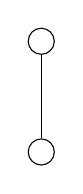
\begin{tikzpicture}[every tree node/.style={draw,circle},sibling distance=10pt, level distance=40pt]
\tikzset{edge from parent/.style={draw, edge from parent path=
    {(\tikzparentnode) -- (\tikzchildnode)}}}
    \Tree [.{} [.{} ] ] 
\end{tikzpicture} \hspace{1.5em}
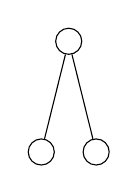
\begin{tikzpicture}[every tree node/.style={draw,circle},sibling distance=10pt, level distance=40pt]
\tikzset{edge from parent/.style={draw, edge from parent path=
    {(\tikzparentnode) -- (\tikzchildnode)}}}
    \Tree [.{} [.{} ] [.{} ] ] 
\end{tikzpicture}\hspace{1.5em}
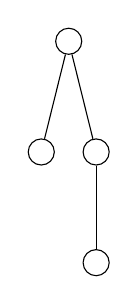
\begin{tikzpicture}[every tree node/.style={draw,circle},sibling distance=10pt, level distance=40pt]
\tikzset{edge from parent/.style={draw, edge from parent path=
    {(\tikzparentnode) -- (\tikzchildnode)}}}
    \Tree [.{} [.{} ] [.{} [.{} ] ] ] 
\end{tikzpicture}\hspace{1.5em}
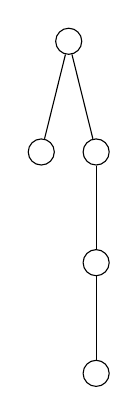
\begin{tikzpicture}[every tree node/.style={draw,circle},sibling distance=10pt, level distance=40pt]
\tikzset{edge from parent/.style={draw, edge from parent path=
    {(\tikzparentnode) -- (\tikzchildnode)}}}
    \Tree [.{} [.{} ] [.{} [.{} [.{} ] ] ] ] 
\end{tikzpicture}

    \cprotect\caption{The initial trees returned by \verb$get_initial_tree$ in \verb$coolOtree$ with $t=1,2,3,$ and $4$ \\
    Note the convenient feature that for each tree, O is equal to \verb$root->left_child->right_sibling$
    }
    \label{exampleotree}
\end{figure}



\begin{figure}
    \centering
    \begin{subfigure}[t]{.49 \textwidth}
	\begin{center}
	    \begin{algorithm}[H] % What does the H do? it makes it work.
	    \begin{algorithmic}
    \Function{cool-ordered-trees}{$t$}
        % \vspace{0.75em}
        \LineComment{Generate initial tree} % TODO
	\State $O\gets root.lchild$
	\State \visit{root}
        \While{$O \ne NULL$}
	    \State $P \gets O.parent$
	    \If{$O.lchild \ne NULL$}
		\State $\pushchild{O}{\popchild{P}}$
		\State $O \gets O.lchild.rsibling$
	    \Else
		\If{$O.parent == root$}
		\State $\pushchild{O}{\popchild{P}}$
		\Else
		\State $\pushchild{O}{\popchild{P}}$
		\State $\pushchild{root}{\popchild{P}}$
		\EndIf
		\State $O \gets O.rsibling$
	    \EndIf
	\State \visit{root}
        \EndWhile
    \EndFunction
	    \end{algorithmic}
    \caption*{Generate all ordered trees with $t+1$ nodes}
	\end{algorithm}
	\end{center}
	% \caption{Pseudoc}
	\label{fig:}
    \end{subfigure}
    \begin{subfigure}[t]{.5 \textwidth}
	\begin{center}
	    \vspace{.9em} % fun alignment
	    % \vspace{2.1em} % fun alignment
\begin{Verbatim}[commandchars=\\\[\]]

void coolOtree(int t, void (*visit)(node*)){
    node* root = get_initial_tree(t);
    node* o=root->left_child->right_sibling;
    visit(root);
    while(o){
	node* p = o->parent;
	if(o->left_child){ 
	    pushchild(o,popchild(p));
	    o=o->left_child->right_sibling;
	}else{
	    if(o->parent == root){ 
		pushchild(o,popchild(p));
	    }else{ 
		pushchild(p->parent,popchild(p));
		pushchild(root,popchild(p));
	    }
	    o=o->right_sibling;
	}
	visit(root);
    }
}
\end{Verbatim}
	\end{center}
	% \caption{ $C$ implementation of coolOtree} 
	\label{fig:}
    \end{subfigure}

    % TODO: change bit colors
    \cprotect\caption{Pseudocode and C implementation}
    \label{fig:otreeCode}
\end{figure}


%%%%%%%%%%%%%%%%%%%%%%%%%%%%%%%%%% ABOVE HERE IS GOOD %%%%%%%%%%%%%%%%%%%%%%%%%%%%%%%%%%%%%%%%

% \chapter{Lattice Paths: Lukasiewicz, Motzkin, Schroder}
TODO: this needs to be organized, could use some figures too.

Motzkin, Schröder, and Łukasiewicz paths provide generalizations of Dyck words.  

Recall the interpretation of Dyck words as paths in the Cartesian plane from Section \ref{sec:Dycks}.

Motzkin paths allow for (1,0) horizontal steps in addition to (1,1) and (1,-1) steps. Schröder paths are identical to Motzkin paths except they allow for $(2,0)$ horizontal steps instead of $(1,0)$.  Łukasiewicz paths allow (1,-1) steps, (1,0) steps and any (1,k) step where k is a positive integer.  All three languages retain the requirement that the path start at the origin, end on the x axis, and never step below the x axis. 

These paths can be encoded in a number of different ways.  In a \emph{-1-based encoding}, each $(1,i)$ step is encoded as i, and every prefix must have a nonnegative sum.  In a \emph{0-based encoding}, each $(1,i)$ step is encoded as $i+1$, and the sum of every prefix must be as large as its length. We primarily use the 0-based encoding. See Fig. \ref{fig:paths}  for examples of these paths using the 0-based encoding.

We refer to Motzkin, Schröder, and Lukasiewicz paths ending at $(n,0)$ as paths of \emph{order n}.  This contrasts slightly with the classification of Dyck words of order n, which terminate at $(2n,0)$

In the context of fixed-content generation, Motzkin and Schröder paths are identical:  Both will have northeast steps encoded as twos, horizontal steps encoded as ones, and southeast steps encoded as zeroes.  However, their Cartesian plane representations will differ in the length of horizontal steps. Notably, Łukasiewicz are a generalization of Motzkin paths, as any Motzkin path is also a Lukasiewicz path.

\begin{figure}[]
	\centering
	\includegraphics[width = .95 \textwidth]{paths.png}
	\caption{}
	\label{fig:paths}
\end{figure}


The number of Dyck words with n zeroes and n ones are counted by the $n\thh$ Catalan number.  Similarly, the number of Motzkin and Schröder paths of order $n$ are counted by the $n\thh$ Motzkin and big Schröder number respectively. The number of Lukasiewicz paths of order $n$ are counted by the $n-1\thh$ Catalan number. % TODO: is this right?
Motzkin, Schröder, and Lukasiewicz paths bear a number of interesting bijective correspondences with other combinatorial objects. Richard Stanely's \emph{Catalan Objects} outlines hundreds of interesting examples.  

Lukasiewicz paths  of order $n$ bear a particularly nice correspondence to rooted ordered trees with $n$ nodes. See Fig. \ref{trees} for an illustration of this.

\begin{figure}[]
	\centering
	\includegraphics[width = .95 \textwidth]{trees.png}
	\caption{The $\mathcal{C}_4$=14 Lukasiewicz paths of order $n=4$ are in bijective correspondence with the 14 rooted ordered trees with $n+1=5$ nodes.  Given a tree, the corresponding word is obtained by recording the number of children of each node in preorder traversal; the zero from the rightmost leaf is omitted.  For example, the two trees in the middle section correspond to 2200 (top) and 2020 (bottom) respectively.}
	\label{trees}
\end{figure}

% TODO: bijections, mirror chapter 2



\chapter{Loopless Motzkin Word Generation}

\subsection{Loopless Motzkin Generation}
Since Lukasiewicz words are a generalization of Motzkin words, the same algorithm can be used to generate Motzkin words by restricting the content set S to be strictly zeroes, ones, and twos.  However, the additional restrictions on Motzkin words allow for a simpler implementation of the rule.   Pseudocode for loopless generation of Motzkin words is given below in Fig. \ref{motzkinAlg}. Further investigation may uncover a similar loopless implementation for the more general Lukasiewicz successor rule.



% \iffalse
\begin{figure}
    \centering
        \begin{algorithm}[H]
        \begin{algorithmic}
        \Function{coolMotzkin}{$s,t$}
        \EndFunction{}
         
        \State $n \gets 2*s+t$
        \State $b \gets 2^1 0^1 2^{s-1} 1^t 0^{s-1}$
        \State $x \gets 3$
        \State $y \gets 2$
        \State $z \gets 2$
        
        \State \visit{$b$}
        
        \While{$x <= n$}
            \State $q \gets b_{x-1}$
            \State $r \gets b_x$
            \vspace{.4em} 
            \State $b_x\gets b_{x-1}$
            \State $b_y\gets b_{y-1}$
            \State $b_z\gets b_{z-1}$
            \State $b_1\gets r$
            \vspace{.4em} 
            \State $x \gets x+1$
            \State $y \gets y+1$
            \State $z \gets y+1$
            
            \vspace{.4em} 
            \If{$b_x = 0$}
                \If{$z-2 > x-y$}
                    \State $b_1=2$
                    \State $b_2=0$
                    \State $b_x=r$
                    \State $x \gets 3$
                    \State $y \gets 2$
                    \State $z \gets 2$
                \Else 
                    \State $x \gets x+1$
                
                \EndIf
                \ElsIf{$q \ge b[x]$}
                    \State $b_x \gets 2$     
                    \State $b_{x-1} \gets 1$     
                    \State $b_1 \gets 1$     
                    \State $z \gets 1$     
                
            \EndIf
            \visit{$b$}
        \EndWhile
        \end{algorithmic}
        % I don't know how to get rid of this "a" here
        \caption{Motzkin}
        \end{algorithm}
    \caption{Pseudocode algorithm for loopless enumeration of Motzkin words}
    \label{motzkinAlg}
\end{figure}
% \fi


\chapter{Loopless (?) Lukasiewicz Word Generation}
\subsection{Lukasiewicz Path Successor Rule}
The successor rule for Lukasiewicz paths is as follows:

Let $S$ be a multiset whose sum is equal to its length.  Let $\mathcal{L}(S)$ denote the set of valid Lukasiewicz words with content equal to S. Let $\alpha \in \mathcal{L}(S)$.  

Let $m$ be the maximum value such that $\alpha_{i-1} \ge \alpha_{i}$ for all $2 \le i \le m$. In other words, let m be the length of the non-increasing prefix of $\alpha$.


\begin{equation*}
    \overleftarrow{\text{luka}}(\alpha) = \begin{cases}
	\leftshift{n}{2} & $if $ m=n \\
	\leftshift{m+1}{1} & $if $ m=n-1 $ or $ \alpha_{m} < \alpha_{m+2}  $ or$ \\
    & (\alpha_{m+2} = 0 $ and $ \sum \rho = m) \\
	\leftshift{m+2}{1} & $ if $ \alpha_{m+2} \neq 0 \\
	\leftshift{m+2}{2} & $otherwise$  \\
\end{cases}
\end{equation*}
In addition to generating Lukasiewicz words, this successor rule also 


\chapter{Final Remarks}
\section{Summary}
\section{Open Problems}

\bibliographystyle{alpha}
\bibliography{sample}

\end{document}
